%% ------------------------------------------------------------------------- %%
\chapter{Implementação}
\label{cap:implementacao}

\section{Ambiente e ferramentas}
- python
- jupyter notebooks
- astropy (falar sobre fits)
- numpy
- matplotlib
- funcoes do utils (compilado de funcoes, falar sobre cada uma)
- dados fits

\section{Notebooks}
% Embora neste exemplo tenhamos apenas um capítulo,  entre a introdução
% e a conclusão de uma monografia podemos ter uma sequência de capítulos
% descrevendo o trabalho e os resultados. Estes podem descrever
% fundamentos, trabalhos relacionados, método/modelo/algoritmo proposto,
% experimentos realizados, resulatdos obtidos.

% Cada capítulo pode ser organizado em seções, que por sua vez pode
% conter subseções. 

% Um exemplo de figura está na figura~\ref{fig:graph}.
% \begin{figure}[htb]a
% 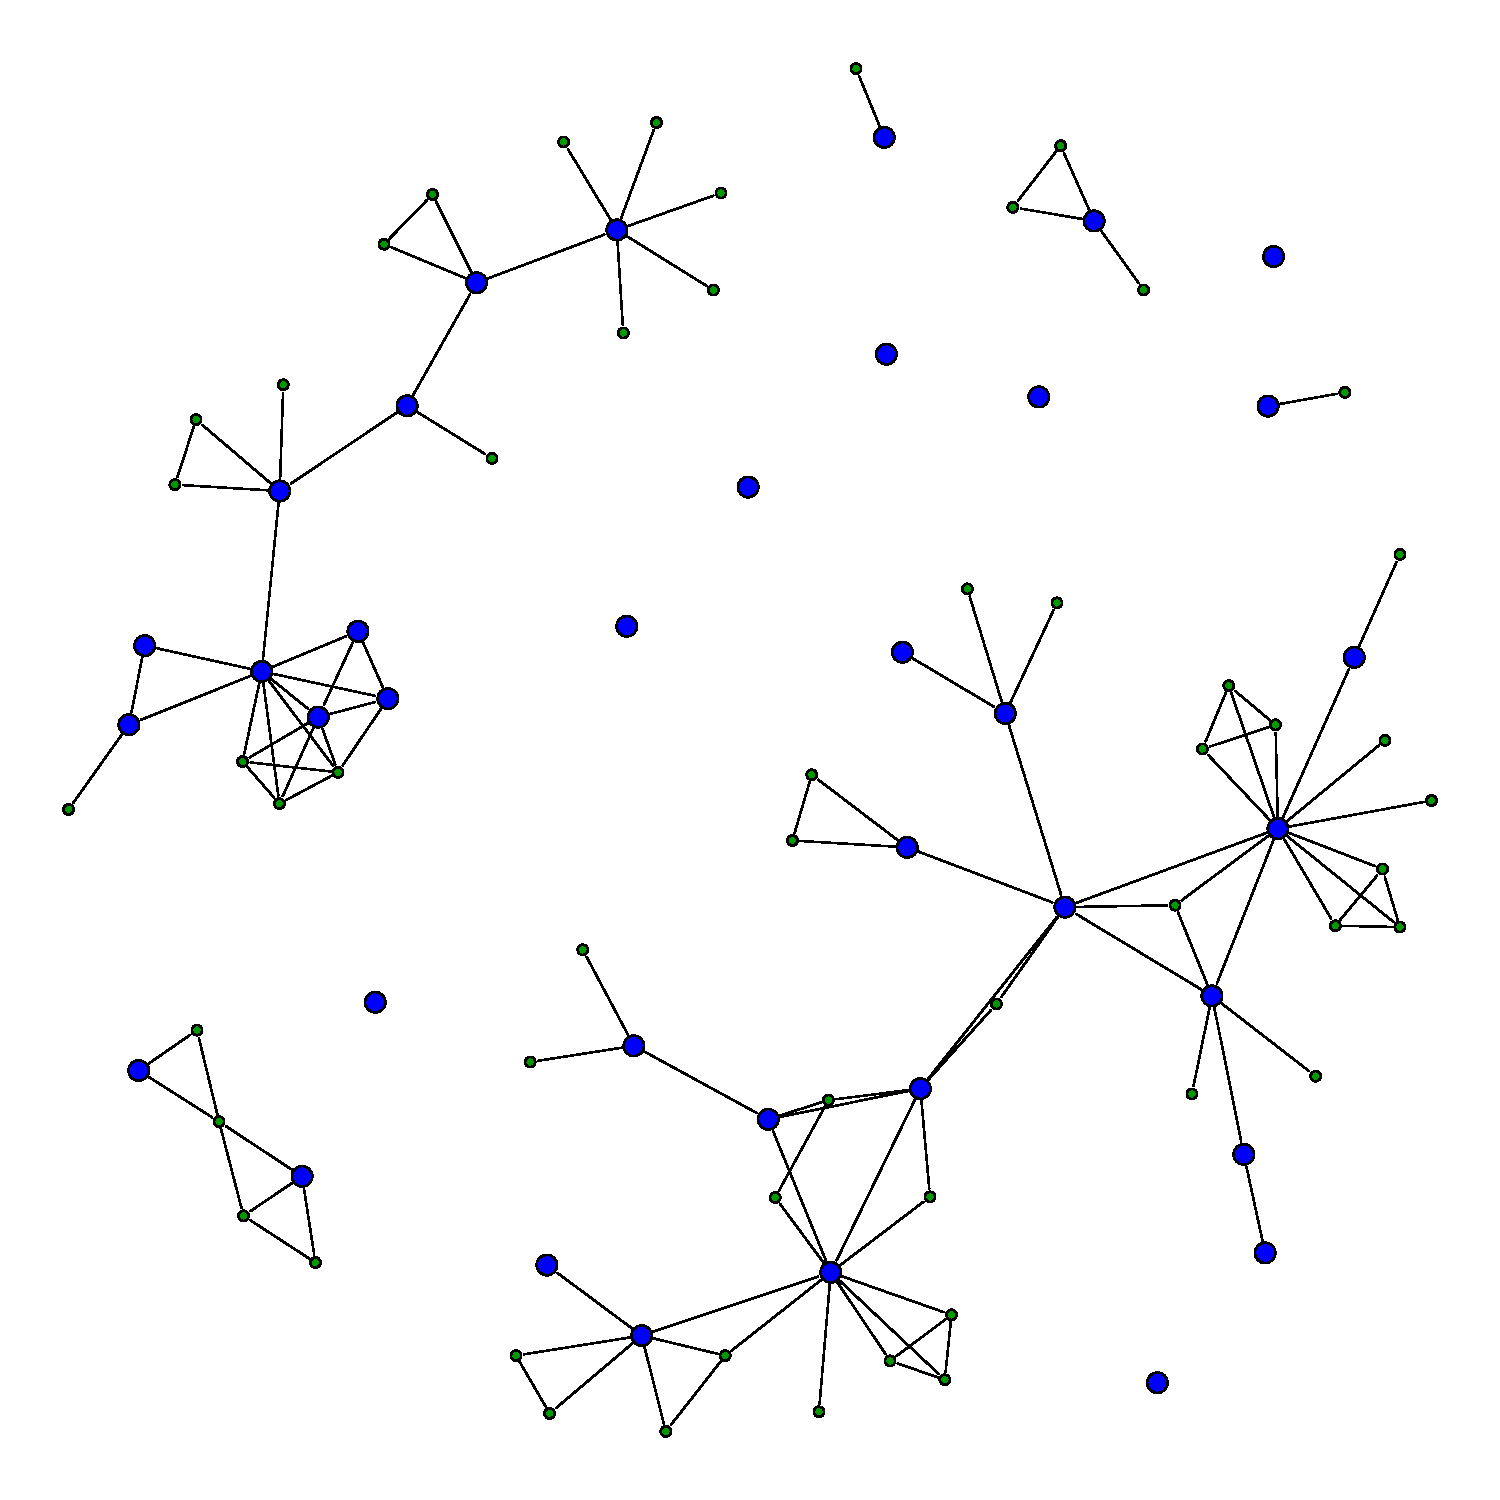
\includegraphics[width=5cm]{figuras/graph}
% \caption{\label{fig:graph}Exemplo de uma figura.}
% \end{figure}
